%!TEX root = ../thesis.tex
%*******************************************************************************
%****************************** Second Chapter *********************************
%*******************************************************************************

\chapter{Methods, Models and Hypothesis testing}

\ifpdf
    \graphicspath{{Chapter2/Figs/Raster/}{Chapter2/Figs/PDF/}{Chapter2/Figs/}}
\else
    \graphicspath{{Chapter2/Figs/Vector/}{Chapter2/Figs/}}
\fi


\section{Ordination}

Ordination can be thought of as series of operations/transformations performed on a data matrix (samples and species table) with the purpose of representing the relationships between the species and samples as faithfully as possible. These methods are made up of two stages; the data are converted into a dissimilarity/similarity matrix of the samples or species which are subsequently transformed into a lower dimensional space where the interpoint distances are related to the distance matrix through the scaling method used.

Metric scaling methods try to maximise the linear correlation between the distances in the dissimilarity matrix and in the lower dimensional space. Non-metric methods on the other hand aim at maximising rank-order correlation between those distances instead.

Some of the reasons for carrying out ordination are :
\begin{itemize}
\item To make the dissimilarities between the sites or species more evident in a visual manner.
\item To reduce the noise from the data, since the projection of the ordination method used will be of a lower dimensional space.
\item To interpret environmental gradients along the dimensions.
\end{itemize}


Ordination methods can be categorised based on how they use external environmental variables; when the method only considers the sites by species table then it is classified as indirect gradient analysis (or unconstrained ordination), when it takes in to account environmental data from the start then it is classified as direct gradient analysis (or constraint ordination). 

Indirect gradient analysis finds the most important gradients in the sites by species data (or more descriptive dimensions), in the absence of environmental data. After the procedure is complete, environmental gradients can be fitted on the new basis and explore how the variables change with sites or species. Direct gradient analysis on the other hand explores how much environmental variables are related to the variation of species composition across sites, by taking into consideration only the variation that can be explained by the environmental variables. It can be thought of as a regression technique testing the null hypothesis that the species composition is not related to environmental gradients.

%%PCA
\subsection{PCA}
\label{ssec:PCA}
Principal Component analysis (PCA) is a clustering technique that can be used as an ordination method as well. It works by finding the direction that maximises the variance in the data and setting it as the first axis. Then it finds the direction with the second highest explanation of variance that is orthogonal to the first one, and sets it as the second axis, and the direction that is uncorrelated with both the first and the second axis and explains the most variance as the third, and so on. For ordination, since all ecological community data are measured in the same units, the data do not need to be standardised to unit variance, and thus the method involves finding the eigenvectors of the covariance matrix of the data (and not the correlation matrix).

Let the row vector $x_i$ with $p$ columns represent the $i$th sample of our data, with each element denoting how many individual of that particular column (species) where encountered in the sample. We can place the vectors into an $n \times p$ matrix $X$, where $n$ is the number of samples collected. For ecological abundance data we only have to centre the data by finding the mean abundance of each species and subtracting it from matrix $X$:
\begin{align}
\label{eq:columnmean}
u_j &= \frac{1}{n} \sum_{i = 1}^{n} X_{ij} \\
B &= X - h u^T,
\end{align}
where  $u_j$ is the $p\times 1$ vector of mean values, $h$ is a $n \times 1$ vector of ones and $B$ is the centred matrix. This expression can be rewritten by using the $n \times n$ centering matrix $J$ which is defined as
\begin{align}
J = I - \frac{1}{n}O,
\end{align}
where $I$ is the identity matrix and $O$ is $n \times n$ matrix of ones. Multiplying this matrix on the left with $X$ produces the same result as centering the matrix by columns
\begin{equation}
B = JX.
\end{equation}
The $p\times p$ empirical covariance matrix is then computed as
\begin{equation}
C = \frac{B^T B}{n},
\end{equation}
which is diagonalised to find its eigenvectors and eigenvalues 
\begin{equation}
C = VDV^{-1},
\end{equation}
where $D$ is the diagonal matrix with the eigenvalues of $C$ in its diagonal, and $V$ is the matrix with the eigenvectors of $C$ as its columns. The projections of the data onto the eigenvectors is given by 
\begin{equation}
Y = BV.
\end{equation}
To reduce the number of features, we can select the $m$ eigenvectors of $C$ that correspond to the $m$ largest eigenvalues, sort them in decreasing order (so the first column of $V$ corresponds to the eigenvector with the largest eigenvalue, the second column to the second largest eigenvalue and so on), and create a new matrix of the sorted eigenvectors
\begin{align}
W_{ij} = V_{ij} \text{ where i = 1,...,$p$ and j = 1,...,$m$}.
\end{align}
Then the projection to the reduced eigenvector space is given by
\begin{equation}
Y_r = BW,
\end{equation}
which is a $n \times m$ matrix.
%Gramm MAtrix
When the number of features $p$ is greater than the number of observations $n$, it is computationally more efficient to diagonalise the Gram matrix $G$ to find the eigenvectors of $C$
\begin{equation}
\label{eq:gram}
G = \frac{BB^T}{n}.
\end{equation}
The Gram matrix has dimensions $n \times n$ and can be diagonalised to give 
\begin{equation}
G = USU^{-1}.
\end{equation}
In this instance, $U$ columns are the eigenvectors of the Gram matrix. The connection between this diagonalisation and of the Covariance matrix can be seen more clearly through the singular value decomposition of $B$
\begin{equation}
B = U \Sigma V^T,
\end{equation}where $U$ and $V$ are $n \times n$ and $p \times p$ matrices respectively with orthogonal unit vectors as columns. The matrix $\Sigma$ is an $n \times p$ rectangular diagonal matrix of positive numbers, the singular values of $B$. Using this representation of $B$, we can rewrite the covariance and Gram matrix as such
\begin{align}
C &= \frac{B^TB}{n} = \frac{(U\Sigma V^T)^TU\Sigma V^T}{n} = \frac{V\Sigma^T U^TU\Sigma V^T}{n} = \frac{V \Sigma^T\Sigma V^T }{n} \\
G &= \frac{BB^T}{n} = \frac{U\Sigma V^T(U\Sigma V^T)^T}{n} = \frac{U\Sigma V^TV\Sigma^T U^T}{n} = \frac{U\Sigma \Sigma^T U^T}{n}.
\end{align}
Since matrices $U$ and $V$ are orthogonal,  their inverse is equal to their transpose (e.g. $U^{-1} = U^T$). The projection of the centred data onto the eigenvectors of the covariance matrix $C$ can be reformulated using the SVD
\begin{align}
Y = BV = U \Sigma V^T V = U \Sigma.
\end{align}
This reformulation tells us that the projections can also be found using the eigenvectors of the Gram matrix (i.e. the left-singular vectors of $B$). The projection to the reduced $m$-dimensional eigenvector space can be given in a similar manner by
\begin{align}
\label{eq:reducedGram}
Y_r = U_m \Sigma_m,
\end{align}
where $\Sigma_m$ is the matrix of the $m$ largest singular values, and $U_m$ the matrix with their corresponding eigenvectors as columns.

The centred $n \times p$ data matrix $B$ has maximum rank $r$ equal to the minimum of the numbers $n$ and $p$. This means that there are at most $r$ linearly independent row (or columns) vectors, and consequently, at most $r$ singular values in the $n \times p$ matrix $\Sigma$. Comparing the two decompositions of the Covariance and Gram matrix, we note that the matrices $\Sigma^T \Sigma$ and $\Sigma \Sigma^T$ have the same number of non-zero elements in their diagonals, even if they are of dimension $p \times p$ and $n \times n$ respectively. Thus, we can conclude that the Covariance and Gram matrices have the same eigenvalues.

An important assumption of PCA that plays a role in our data, is that it is a linear method. This means that the basis that the data are projected onto is a linear combination of their features. Thus, the projection is essentially a rotation and stretching of the basis set. 

This linear assumption of PCA makes it unsuitable for use in Ecological data sets. The species composition varies non linearly across samples, and the relationship between species is also not linear. The presence of a species in a sample is usually much more important that the actual number of reads of that species. Thus, when the data are projected onto the eigenvectors of the covariance matrix (Figure \ref{fig:pcaotu12}), they are distorted into a horseshoe shape (i.e. like an arch) \cite{Gauch 1982}.

%FIGURE OF PCA
\begin{figure}
\centering
\includegraphics[width = 0.7\textwidth]{"pcaotu12"}
\caption{First 2 dimensions of PCA performed on the full OTU table. The 2 axes account for 47.8\% of the variance.}
\label{fig:pcaotu12}
\end{figure}

%%PCOA
\subsection{PCoA}
A more general method of ordination, of which PCA is a special case, is called Principal Coordinates Analysis (PCoA), otherwise known as classical multidimensional scaling. The method aims to represent distances between samples (in the species space), but in a lower dimension, so that they can be easily interpreted. This is done by creating a distance matrix using whatever metric we wish (with the condition that it returns a scalar given two vectors of arbitrary dimensions) and projecting it to a lower dimensional space by maximising the correlations between the distances in the distance matrix and the distances in the lower dimensional representation. Thus, the method assumes that the distances used are meaningful and thus try to reserve them.

Lets define by $D_{ij}$ the $n \times n$ distance matrix between the samples (rows) in $X$ (where $D_{ij}$ indicates the distance between the sample $i$ with sample $j$). It is evident from the construction of the matrix that it is symmetric, since the distance between sample $i$ and $j$ is the same the distance between $j$ and $i$. When using a euclidean measure the diagonals of the matrix are zero. The euclidean metric is given by
\begin{align}
D_{ij} = {||\bf{x}_i-\bf{x}_j||^2},
\label{eq:euclideanmetric}
\end{align}
where $\bf{x}_i$ is a row vector of the data matrix $X$ containing the abundance reading for the sample $i$, and $||\cdot||^2$ is the L2 norm.

The algorithm works by double centering the distance matrix, or in other words subtracting the row and column mean, and multiplying it by $-\frac{1}{2}$
\begin{align}
\label{eq:Kmatrix}
K = -\frac{1}{2}JDJ.
\end{align}
Then the matrix $K$ is decomposed into its eigenvectors, which are the columns of matrix $E$, and eigenvalues, which make up the diagonals of matrix $\Lambda$
\begin{equation}
    K = E\Lambda E
\end{equation}

The $m$ largest eigenvalues with their corresponding eigenvectors are collected and sorted in a descending manner in matrices $E_m$ and $\Lambda_m$ (so the largest eigenvalue is $\Lambda_{m,11}$ with corresponding eigenvector $E_{m,{ \bullet}1}$, the first column of the $E_m$ matrix). The projection of the data onto the reduced $m$-dimensional space is given by
\begin{align}
Y_r = E_m \Lambda_m^{(1/2)},
\end{align}
where the exponent is applied elementwise on all eigenvalues (so the square root of the eigenvalues is used). This representation looks very similar to the one obtained in equation \ref{eq:reducedGram}, where the projection is calculated using the eigenvectors of the Gram matrix. We will show how, when using an Euclidean metric, PCoA is equivalent to PCA.

We can expand the euclidean distance matrix into 
\begin{align}
D_{ij} &= ||x_i - x_j||^2 = ||x_i - \bar{x}+\bar{x} -x_j||^2   \\
&= ||x_i - \bar{x}||^2 + ||x_j - \bar{x}||^2 - 2(x_i - \bar{x})\cdot (x_j - \bar{x}),
\end{align}
where the last term is the dot product between the vectors of the mean-centred samples $i$ and $j$. The $||x_i - \bar{x}||^2$ term is an additive constant over the columns of $D_{ij}$, and so is the corresponding term with $x_j$ over the rows of the matrix.  To explore the connection between the last term and the Gram matrix, we have to reformulate the later to an equivalent representation of the first. 


The mean centred matrix $B$ can be visualised as row vectors $x_i - \bar{x}$ stacked on top of each other vertically, where $x_i$ denotes the row vector of data matrix $X$ (i.e. the species abundance of sample $i$) and $\bar{x}$ denotes the row vector with the mean number of reads of each species across all samples
\begin{equation}
\bar{x} = [u_1,u_2,...,u_p], 
\end{equation}
where $u_j$ is defined as in equation \ref{eq:columnmean}. To construct the Gram matrix, we multiply the mean-centred matrix with its transpose
\begin{equation}
\brows{(x_1 - \bar{x})\\(x_2 - \bar{x})\\ \rowsvdots \\(x_n - \bar{x})} \cdot 
\begin{pmatrix}
\vert &\vert&&\vert\\
\text{\begin{sideways}$(x_1 - \bar{x})$
\end{sideways}}&
\text{\begin{sideways}$(x_2 - \bar{x})$
\end{sideways}}& 
\hdots&
\text{\begin{sideways}$(x_n - \bar{x})$
\end{sideways}}\\
\vert&\vert &&\vert 
\end{pmatrix}= 
\begin{pmatrix}
(x_1-\bar{x})\cdot (x_1-\bar{x}) &\hdots&(x_1-\bar{x}) \cdot (x_n-\bar{x}) \\
(x_2-\bar{x}) \cdot (x_1-\bar{x})&\hdots&(x_2-\bar{x}) \cdot (x_n-\bar{x})\\
\vdots&\ddots&\vdots\\
(x_1-\bar{x})\cdot (x_n-\bar{x})&\hdots&(x_n-\bar{x})\cdot (x_n-\bar{x})
\end{pmatrix},
\end{equation}
and get the expression 
\begin{equation}
G_{ij} =(x_i-\bar{x}) \cdot (x_j-\bar{x}). 
\end{equation}
The Gram matrix's rows and columns means are equal to zero since it is double-centred by construction
\begin{align}
G = BB^T = JX(JX)^T = JXX^TJ^T = JG_{uc}J,
\end{align}
where $J$ is the centring matrix (which  is symmetric), and $G_{uc}$ the uncentered Gram matrix. Therefore, when we double centre the Distance matrix, we end up with the Gram matrix scaled by a constant number
\begin{align}
JD_{ij}J&= J\left(||x_i - \bar{x}||^2 + ||x_j - \bar{x}||^2 - 2G_{ij}\right)J \\
&= -2G_{ij}\\
K &= G,
\end{align}
Where $K$ is the matrix we decompose into its eigenvalues and eigenvectors in the PCoA method (equation \ref{eq:Kmatrix}). The two terms preceding the Gram matrix go to zero when double-centred since they are constants over rows and columns. As mentioned earlier, the Gram matrix itself stays the same when double centred since its rows' and columns' mean is zero. 

Therefore, diagonalising the $K$ matrix when using a euclidean distance metric (PCoA method) is equivalent to diagonalising the Gram matrix of the mean-centred data. The projections produced by the two methods are the same since the eigenvector ($E$ for PCoA and $U$ for PCA) and eigenvalue ($\Lambda^{(1/2)}$ for PCoA and $\Sigma $ for PCA) matrices are the same. 

%Other distance metrics
%~~~~~~~~~~~~~~~~~~~~~~~~~~~~~~~~~~~~~~
A Euclidean distance metric, however, is not very useful when it comes to ecological abundance data. This is because it suffers from the same drawbacks that PCA does (see earlier discussion in section \ref{ssec:PCA}). The framework of PCoA was developed so as to enable the use of other measures which are more suitable to ecological data, where the presence of a species in a sample is more important than the number of reads of that species. Such a measure is the bray-curtis dissimilarity statistic, which quantifies how dissimilar two samples are based on species common to both of them. The measure $B_{ij}$ is defined as
%~~~~~~~~~~~~~~~~Bray Curtis
\begin{equation}
    B_{ij} = \frac{\sum_{k =1}^{p} |X_{ik} - X_{jk}|}{\sum_{k =1}^{p} X_{ik} + X_{jk}},
\end{equation}
where $X_{ik}$ is the data matrix which denotes the number of reads of speciment $k$ in sample $i$. The statistic ranges from 0, where the samples have the same species composition, to 1 where the samples do not have any species in common, and is semimetric\footnote{Semimetric measures do not satisfy the triangle inequality.}.

If we use this statistic to calculate the distance matrix $D_{ij}$ and then carry out PCoA, the arch effect is removed from the 2 dimensional ordination plot and can better separate the different river samples. As it can be seen in Figure \ref{fig:pcoaotu12}, the method can separate well samples from the upper Marañón part of the river (yellow points on the upper right corner of the plot). Samples from the other parts are grouped together on the opposite side from the upper Marañón part. Black and white river samples are not very well separated, and occupy the same space (except on the upper right corner where no black water samples are found). Even when the ordination method produces a better spread of results than when using PCA, the variance explained by the first 2 axes is only 19.8\%.


%% PCoA bray curtis.
\begin{figure}[h]
\centering
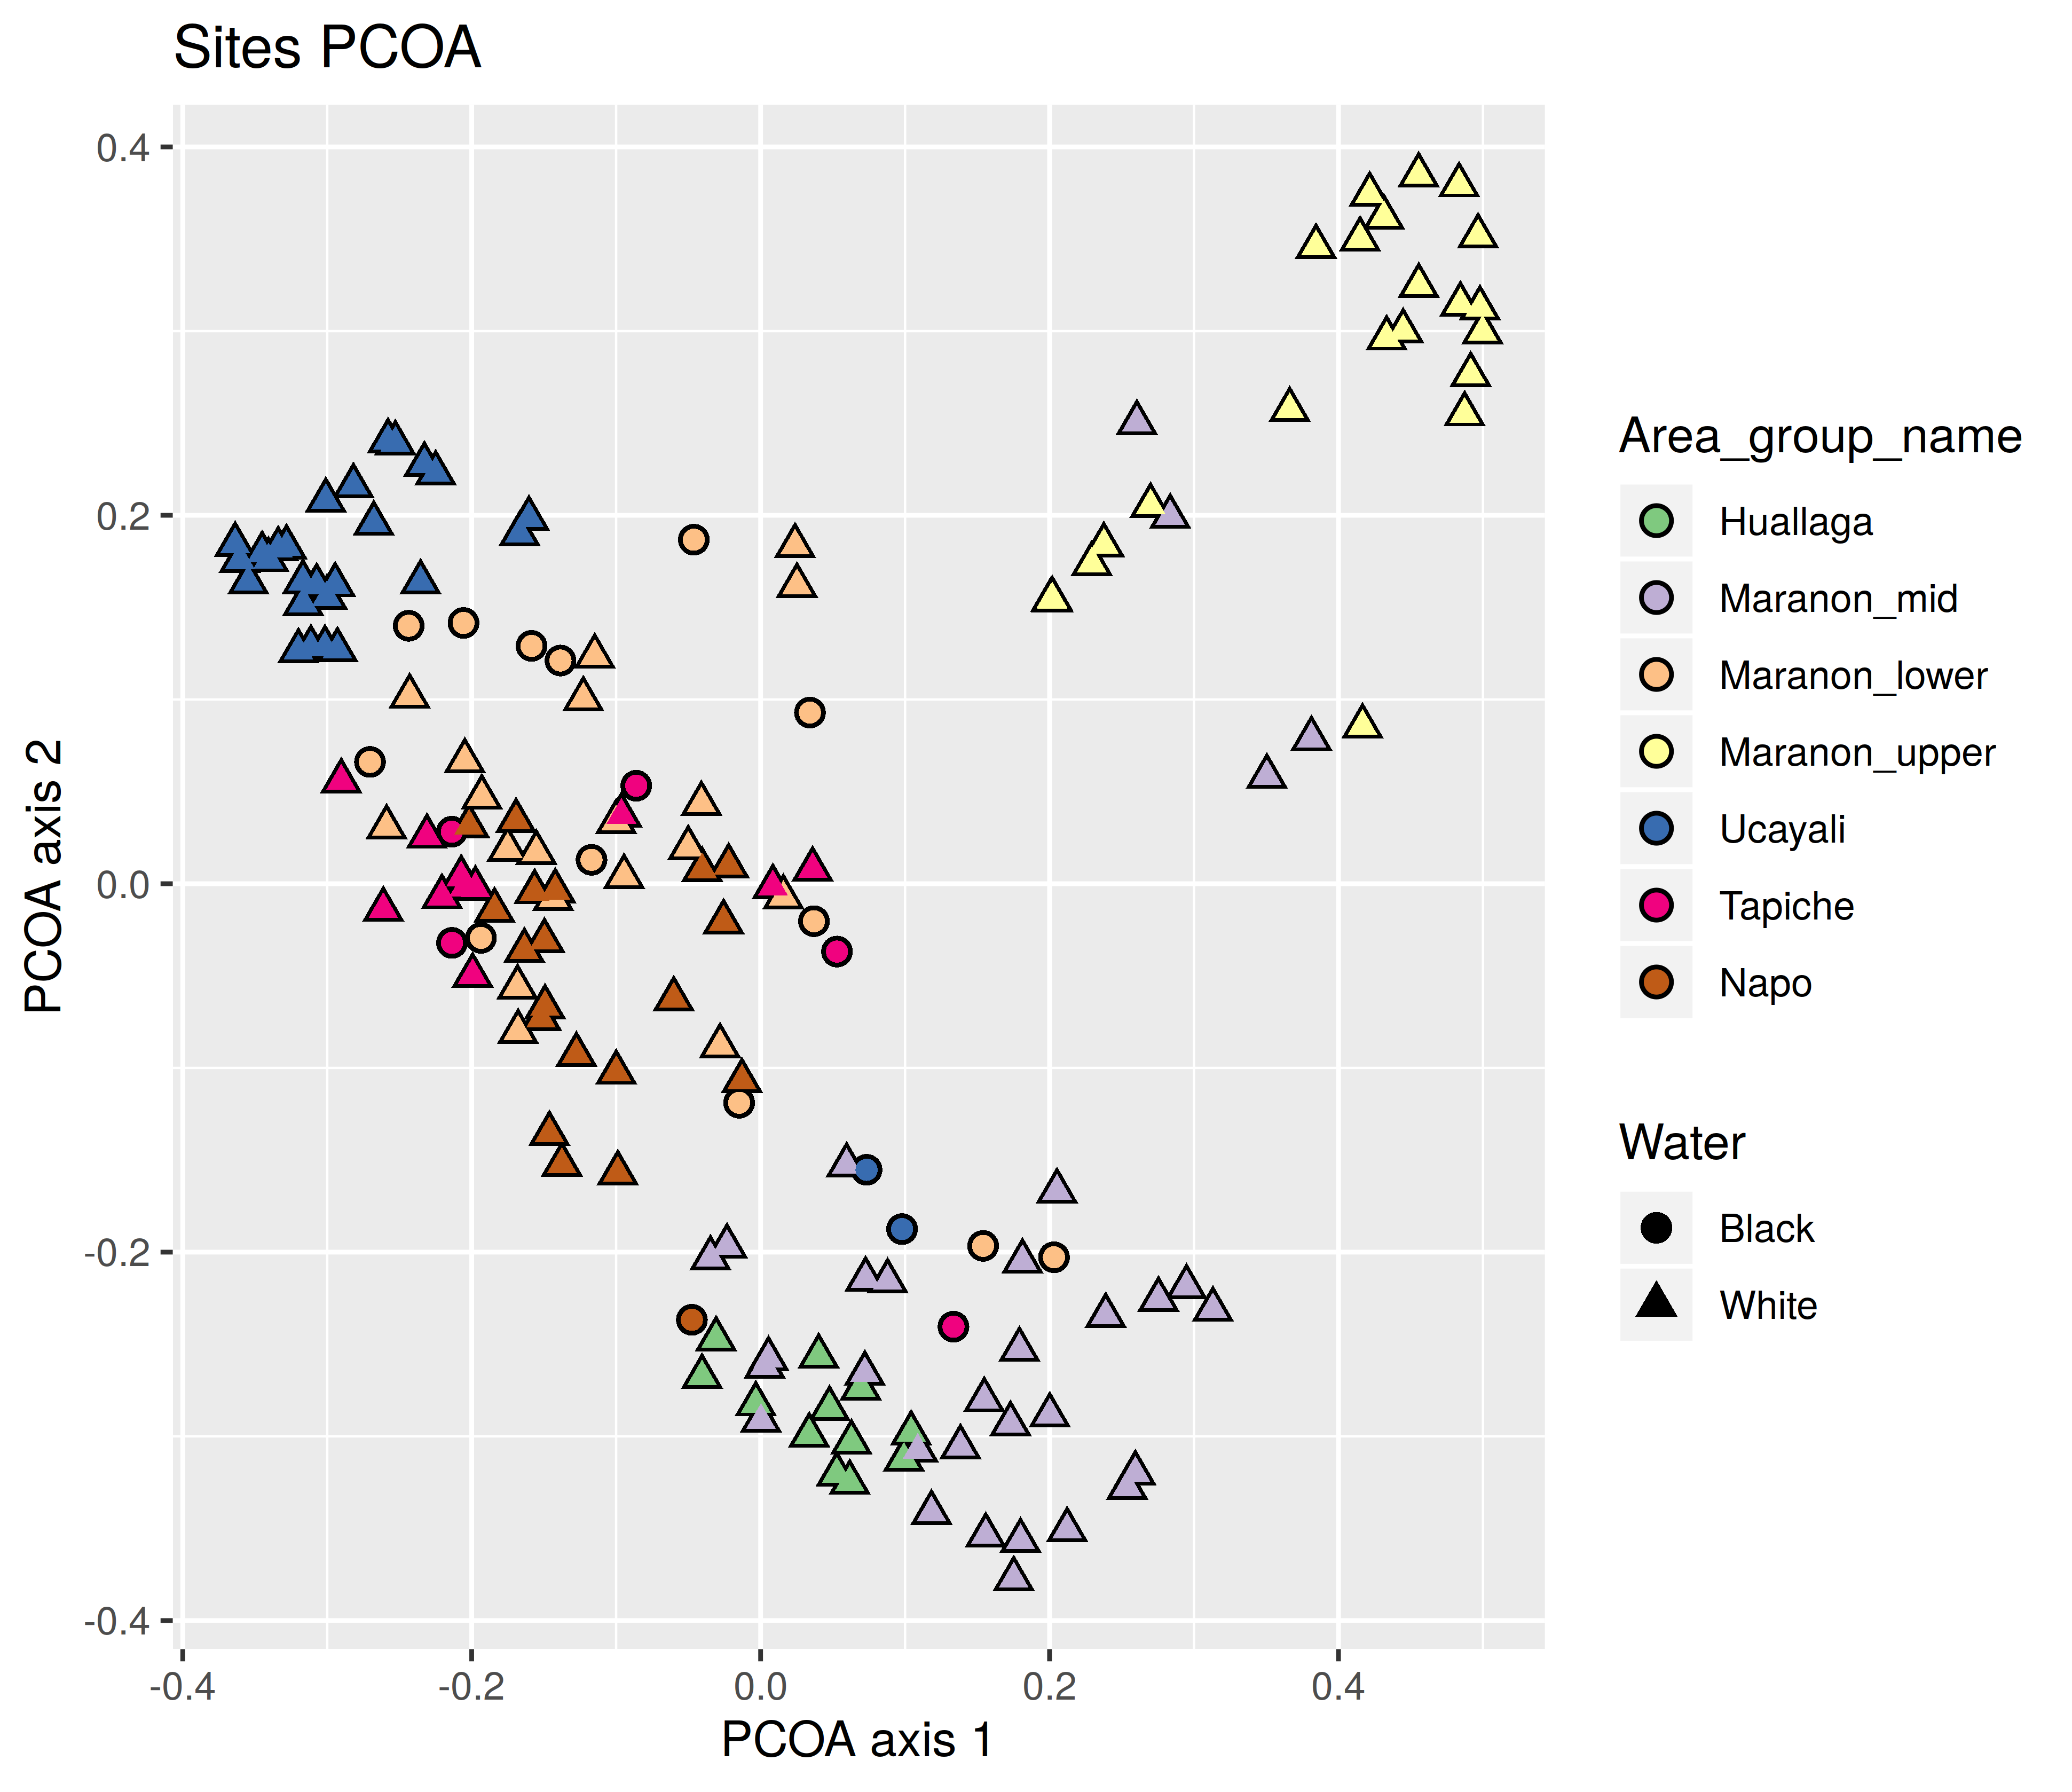
\includegraphics[width = 0.7\textwidth]{pcoaotu12}
\caption{First 2 dimensions of PCoA performed on the full OTU table using the Bray Curtis statistic as the distance metric. The 2 axes account for 19.8\% of the variance.}
\label{fig:pcoaotu12}
\end{figure}

To illustrate the effect of measures on the PCoA algorithm, we produced 2 dimensional ordination plots for the Euclidean and the Jaccard metrics. The Euclidean metric has the form given in equation \eqref{eq:euclideanmetric} and the ordination plot (see Figure \ref{fig:pcoaeuc}) has the same form as the one obtained using PCA. The only difference is the scale (the covariance matrix is divided by the number of samples) and the reflection of the points on the x-axis. The Jaccard metric is given by
\begin{equation}
Jac_{ij} =\frac{2C_{ij}}{1-C_{ij}},
\end{equation} 
where $C_{ij}$ is the Bray-Curtis statistic between sample $i$ and $j$. The ordination plot produced using this index is shown in Figure \ref{fig:pcoajac}.

%%RESULTS of PCoA with different metrics
\begin{figure}[h]
\centering
\begin{subfigure}{0.4\textwidth}
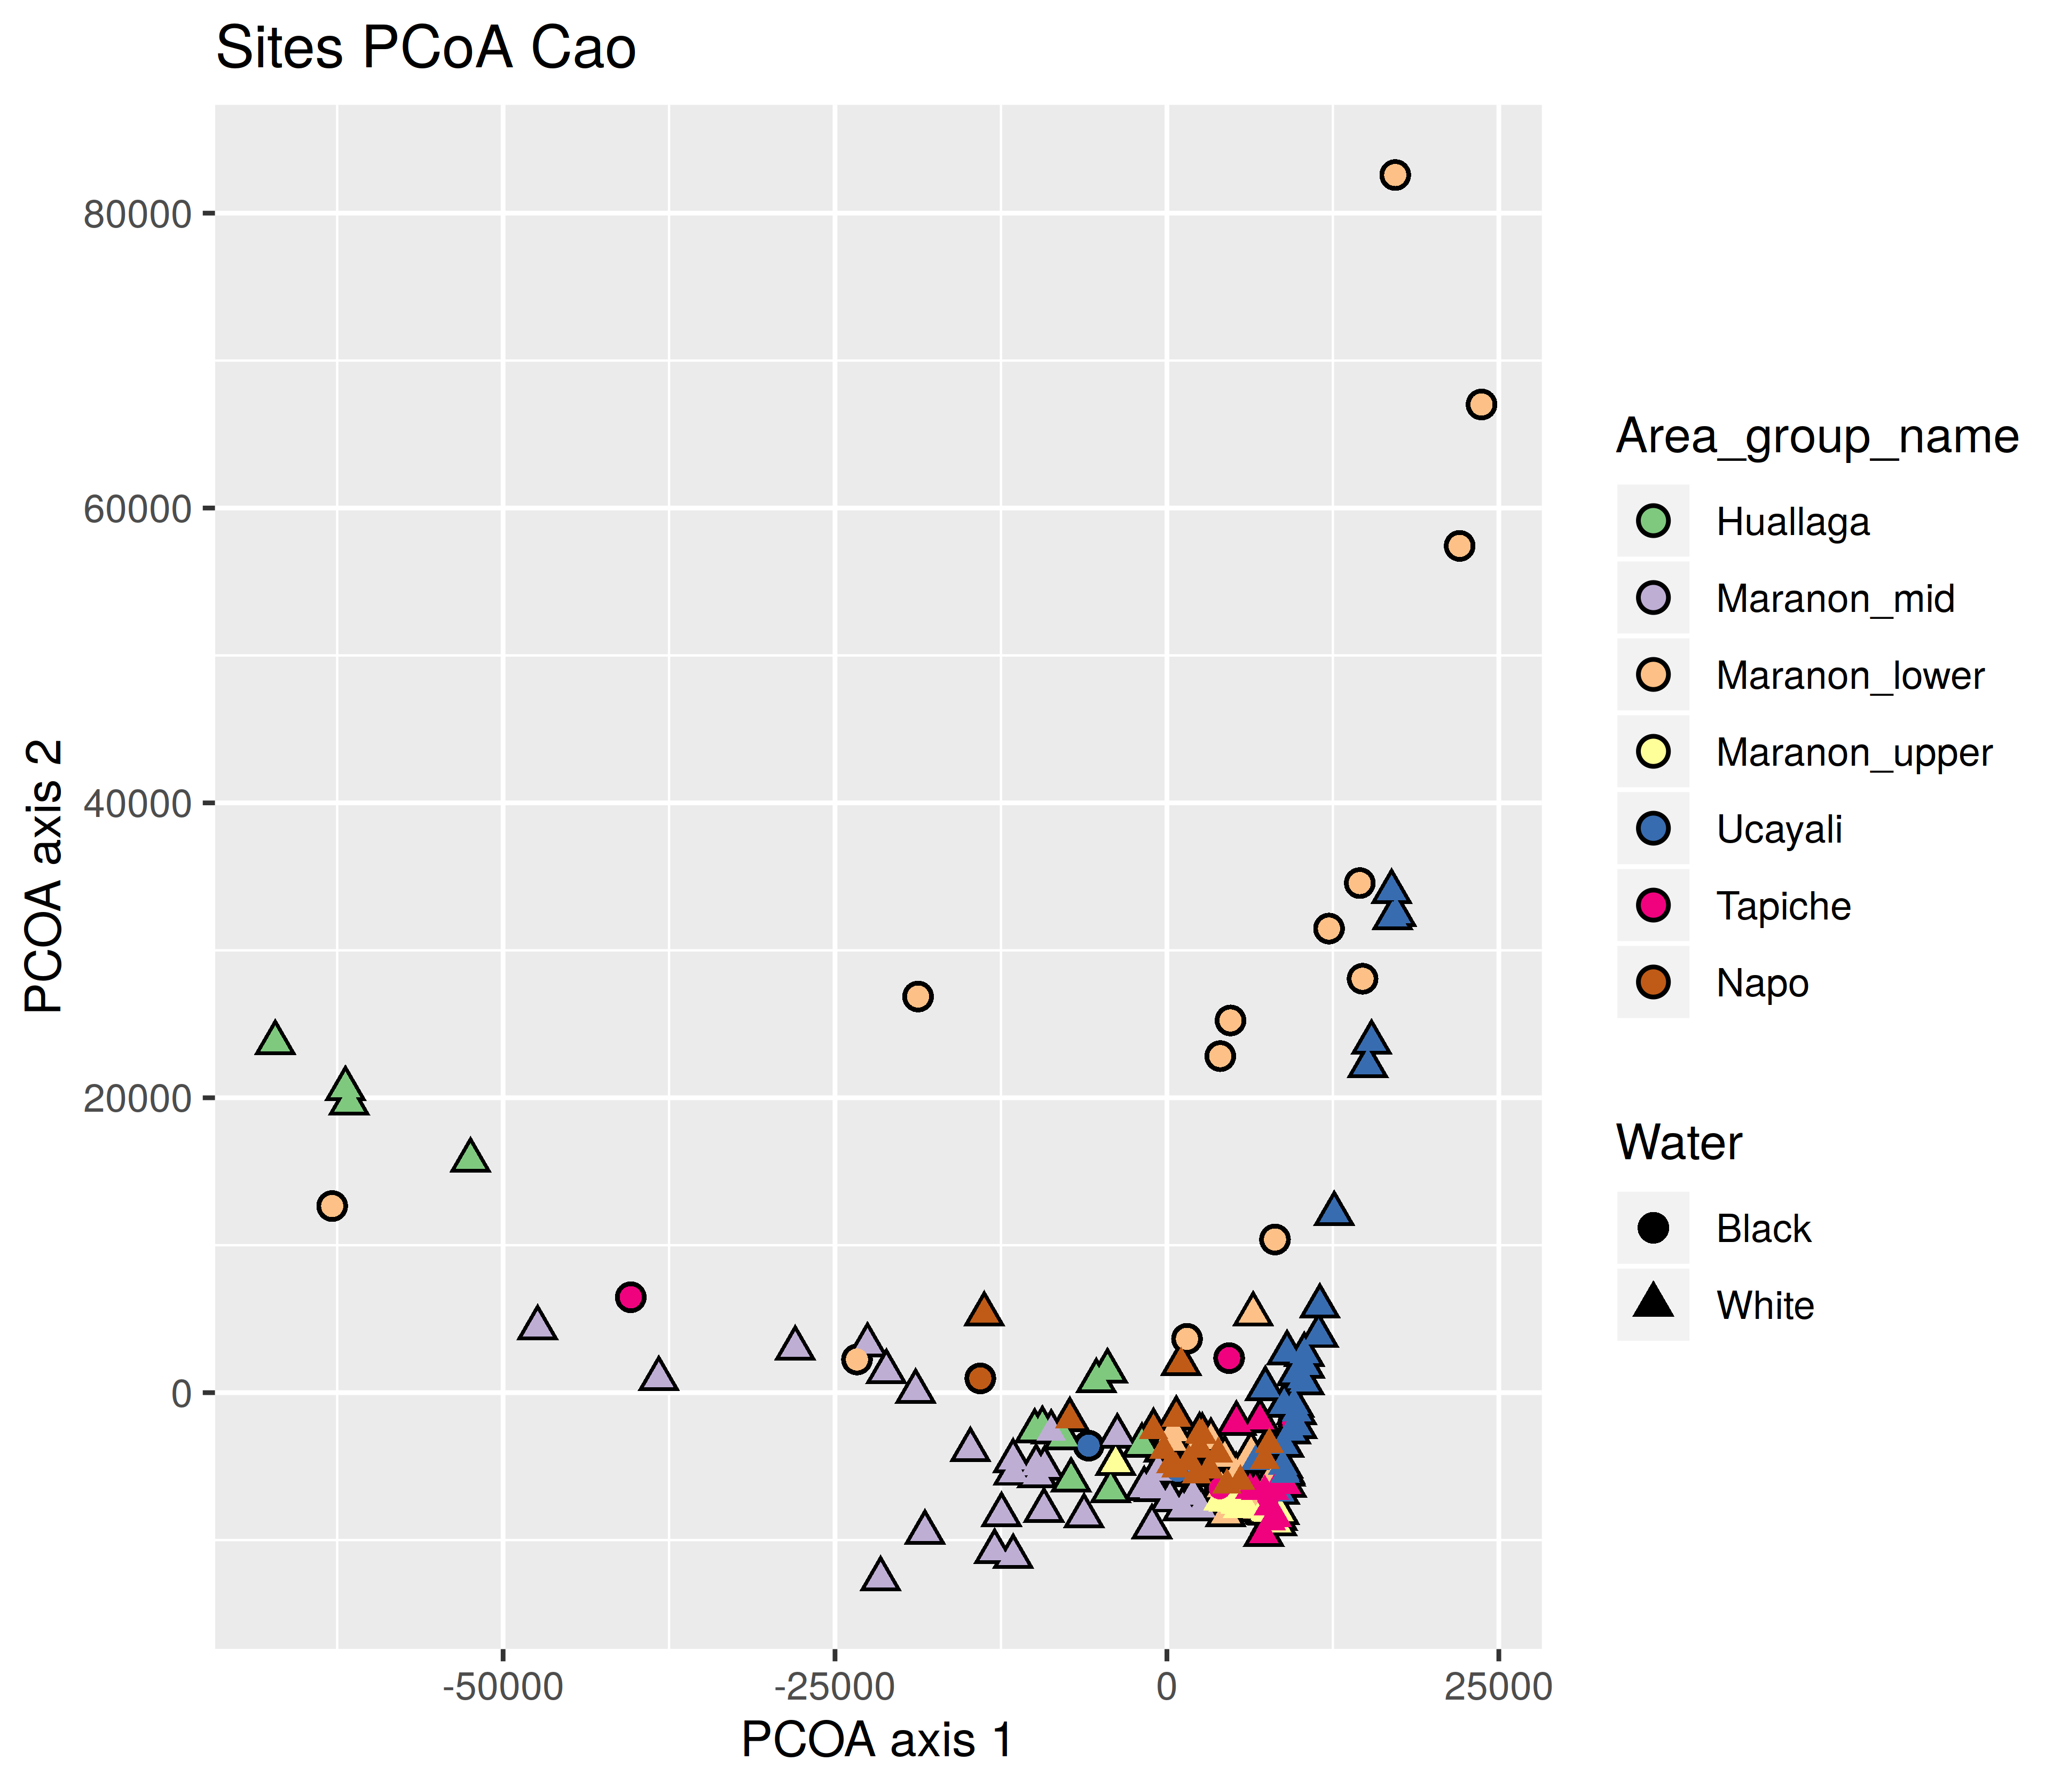
\includegraphics[width = \textwidth]{pcoa12eucotu}
\caption{PCoA using the Euclidean Metric. The result is the same as with PCA; only the scales have different values and the points are flipped over the X-axis.}
\end{subfigure}
\label{fig:pcoaeuc}
\begin{subfigure}{ 0.4\textwidth}
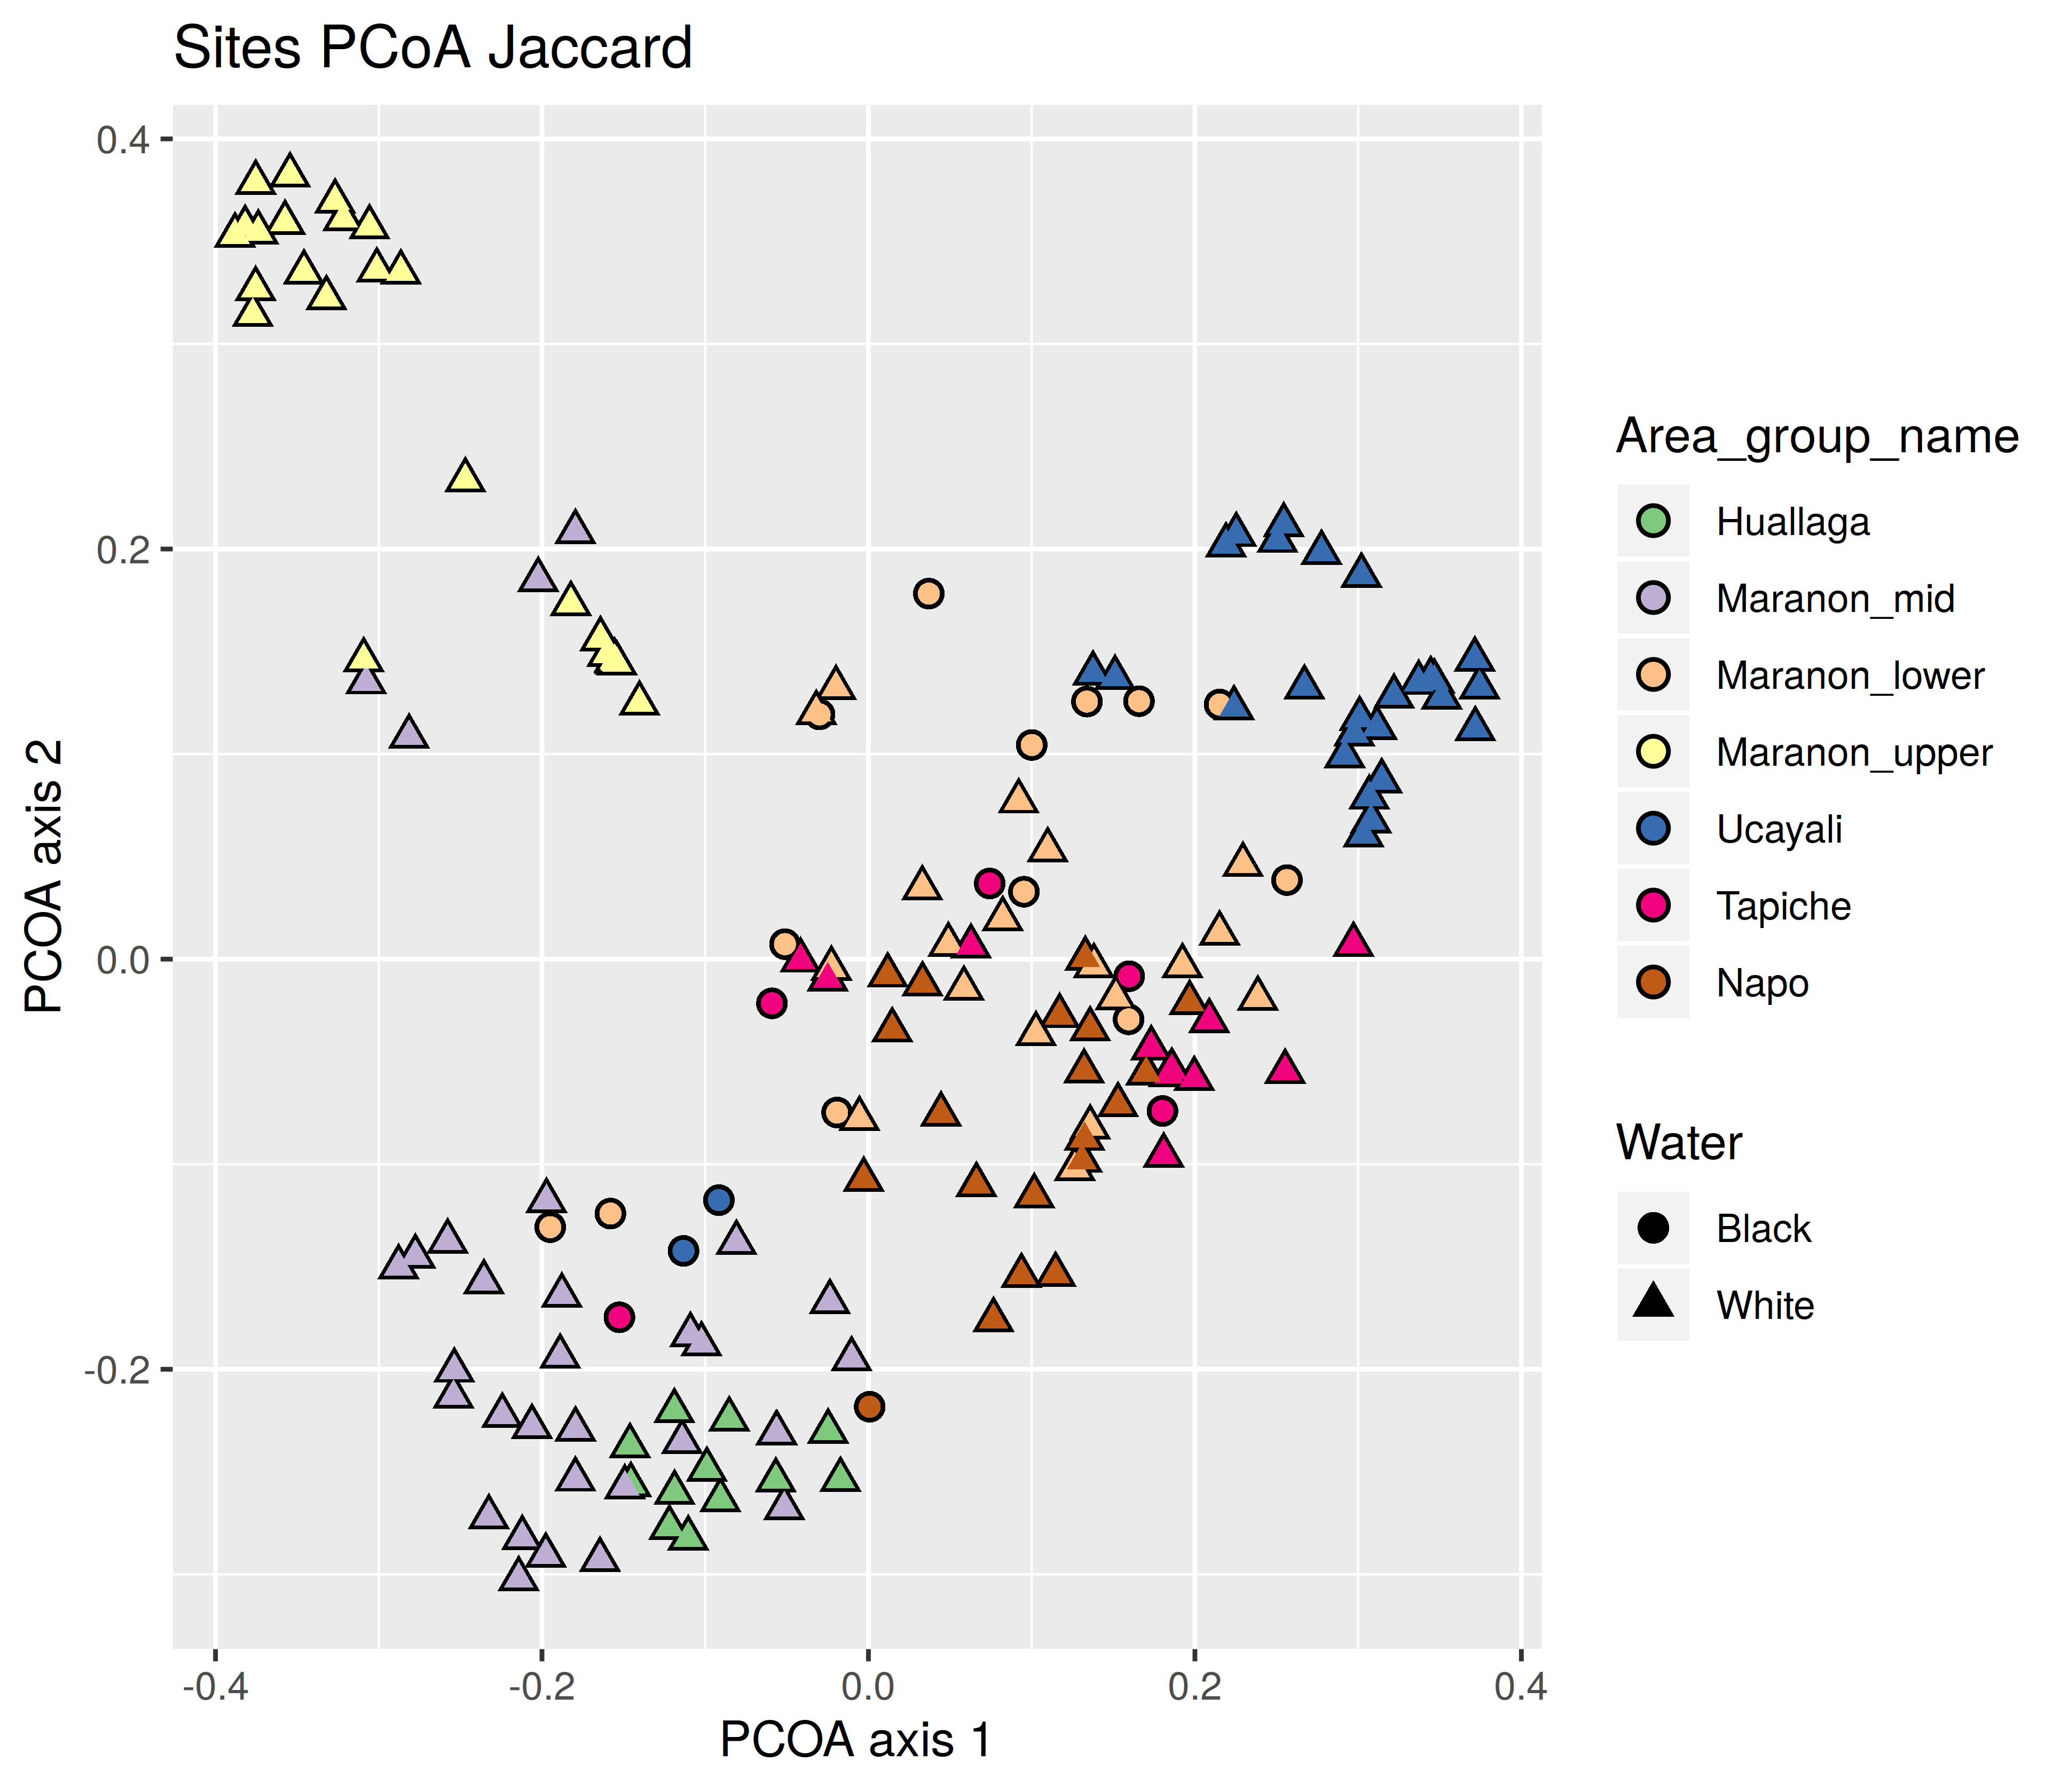
\includegraphics[width = \textwidth]{pcoa12jacotu}
\caption{PCoA using the Jaccard metric. The result is similar with the one obtained using Bray-Curtis. Both measures are rank-order similar.}
\label{fig:pcoajac}
\end{subfigure}
\end{figure}
%Motivate NMDS
%EG actual distances are not that important so NMDS might be more usefull which maximisies correlation
%% NMDS
%%%Explain similarity of NMDS with PCOA

% Uncomment this line, when you have siunitx package loaded.
%The SI Units for dynamic viscosity is \si{\newton\second\per\metre\squared}.
% \begin{figure}[htbp!] 
% \centering    
% \includegraphics[width=1.0\textwidth]{minion}
% \caption[Minion]{This is just a long figure caption for the minion in Despicable Me from Pixar}
% \label{fig:minion}
% \end{figure}
\subsection{NMDS}
\section{Normalisation}
Our data set has a wide range of total reads per sample. This imbalanced could potentially 
\section{PERMANOVA}
\section{Machine Learning}
\subsection{Logistic Regression}
\subsection{Random Forests}
\section{Hypothesis Testing}

Together with the OTU table, our data also include the location of the samples in the rivers (in Easting and Northing coordinates) and in which part of the river they belong to. Because of this location attribute, our samples cannot be said to be independent. Thus, the way we choose to split our data into training and testing sets will surely affect the accuracy of the classifier. For example, testing on a set that is composed of samples maximally distant from the ones in the training set (see Figure \ref{fig:groupsamp}) will produce different results than testing on a set with all samples in close proximity to the ones in the training set (see Figure \ref{fig:stratsampl}).

%% Stratified an group folds for tain test split plot
\begin{figure}[h]
\centering
\begin{subfigure}{0.4\textwidth}
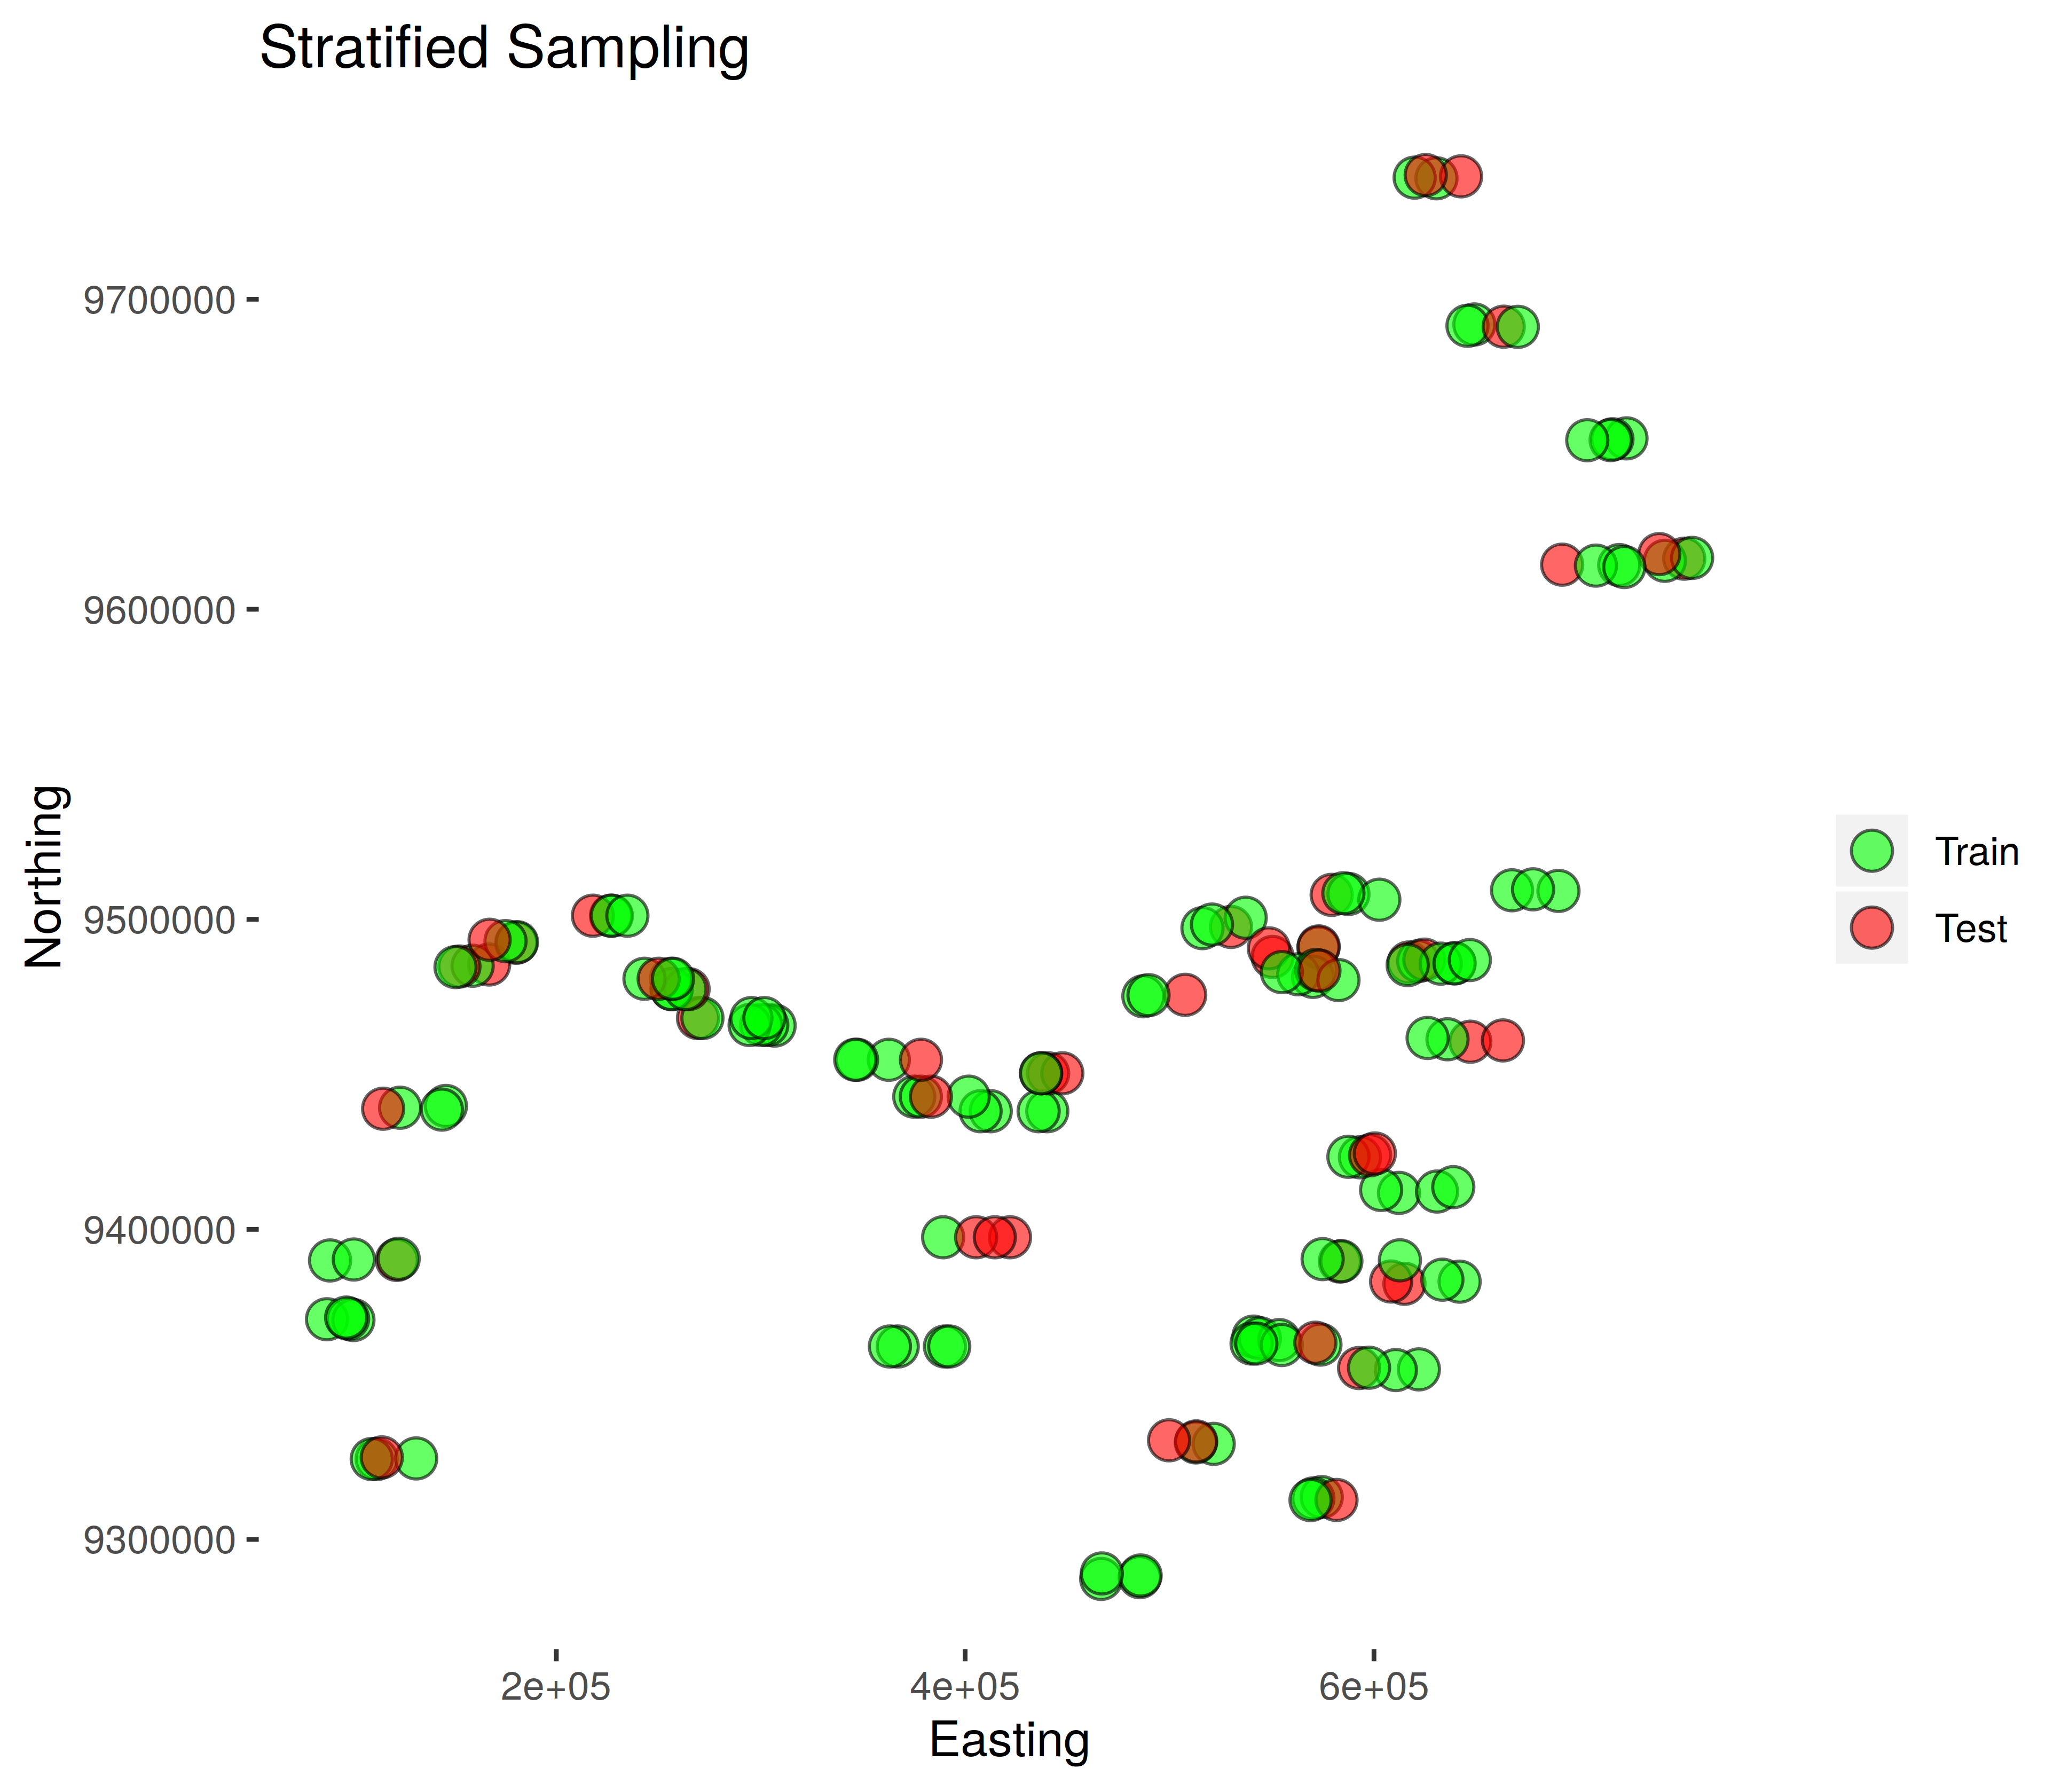
\includegraphics[width = \textwidth]{stratsamp.png}
\end{subfigure}
\begin{subfigure}{0.4\textwidth}
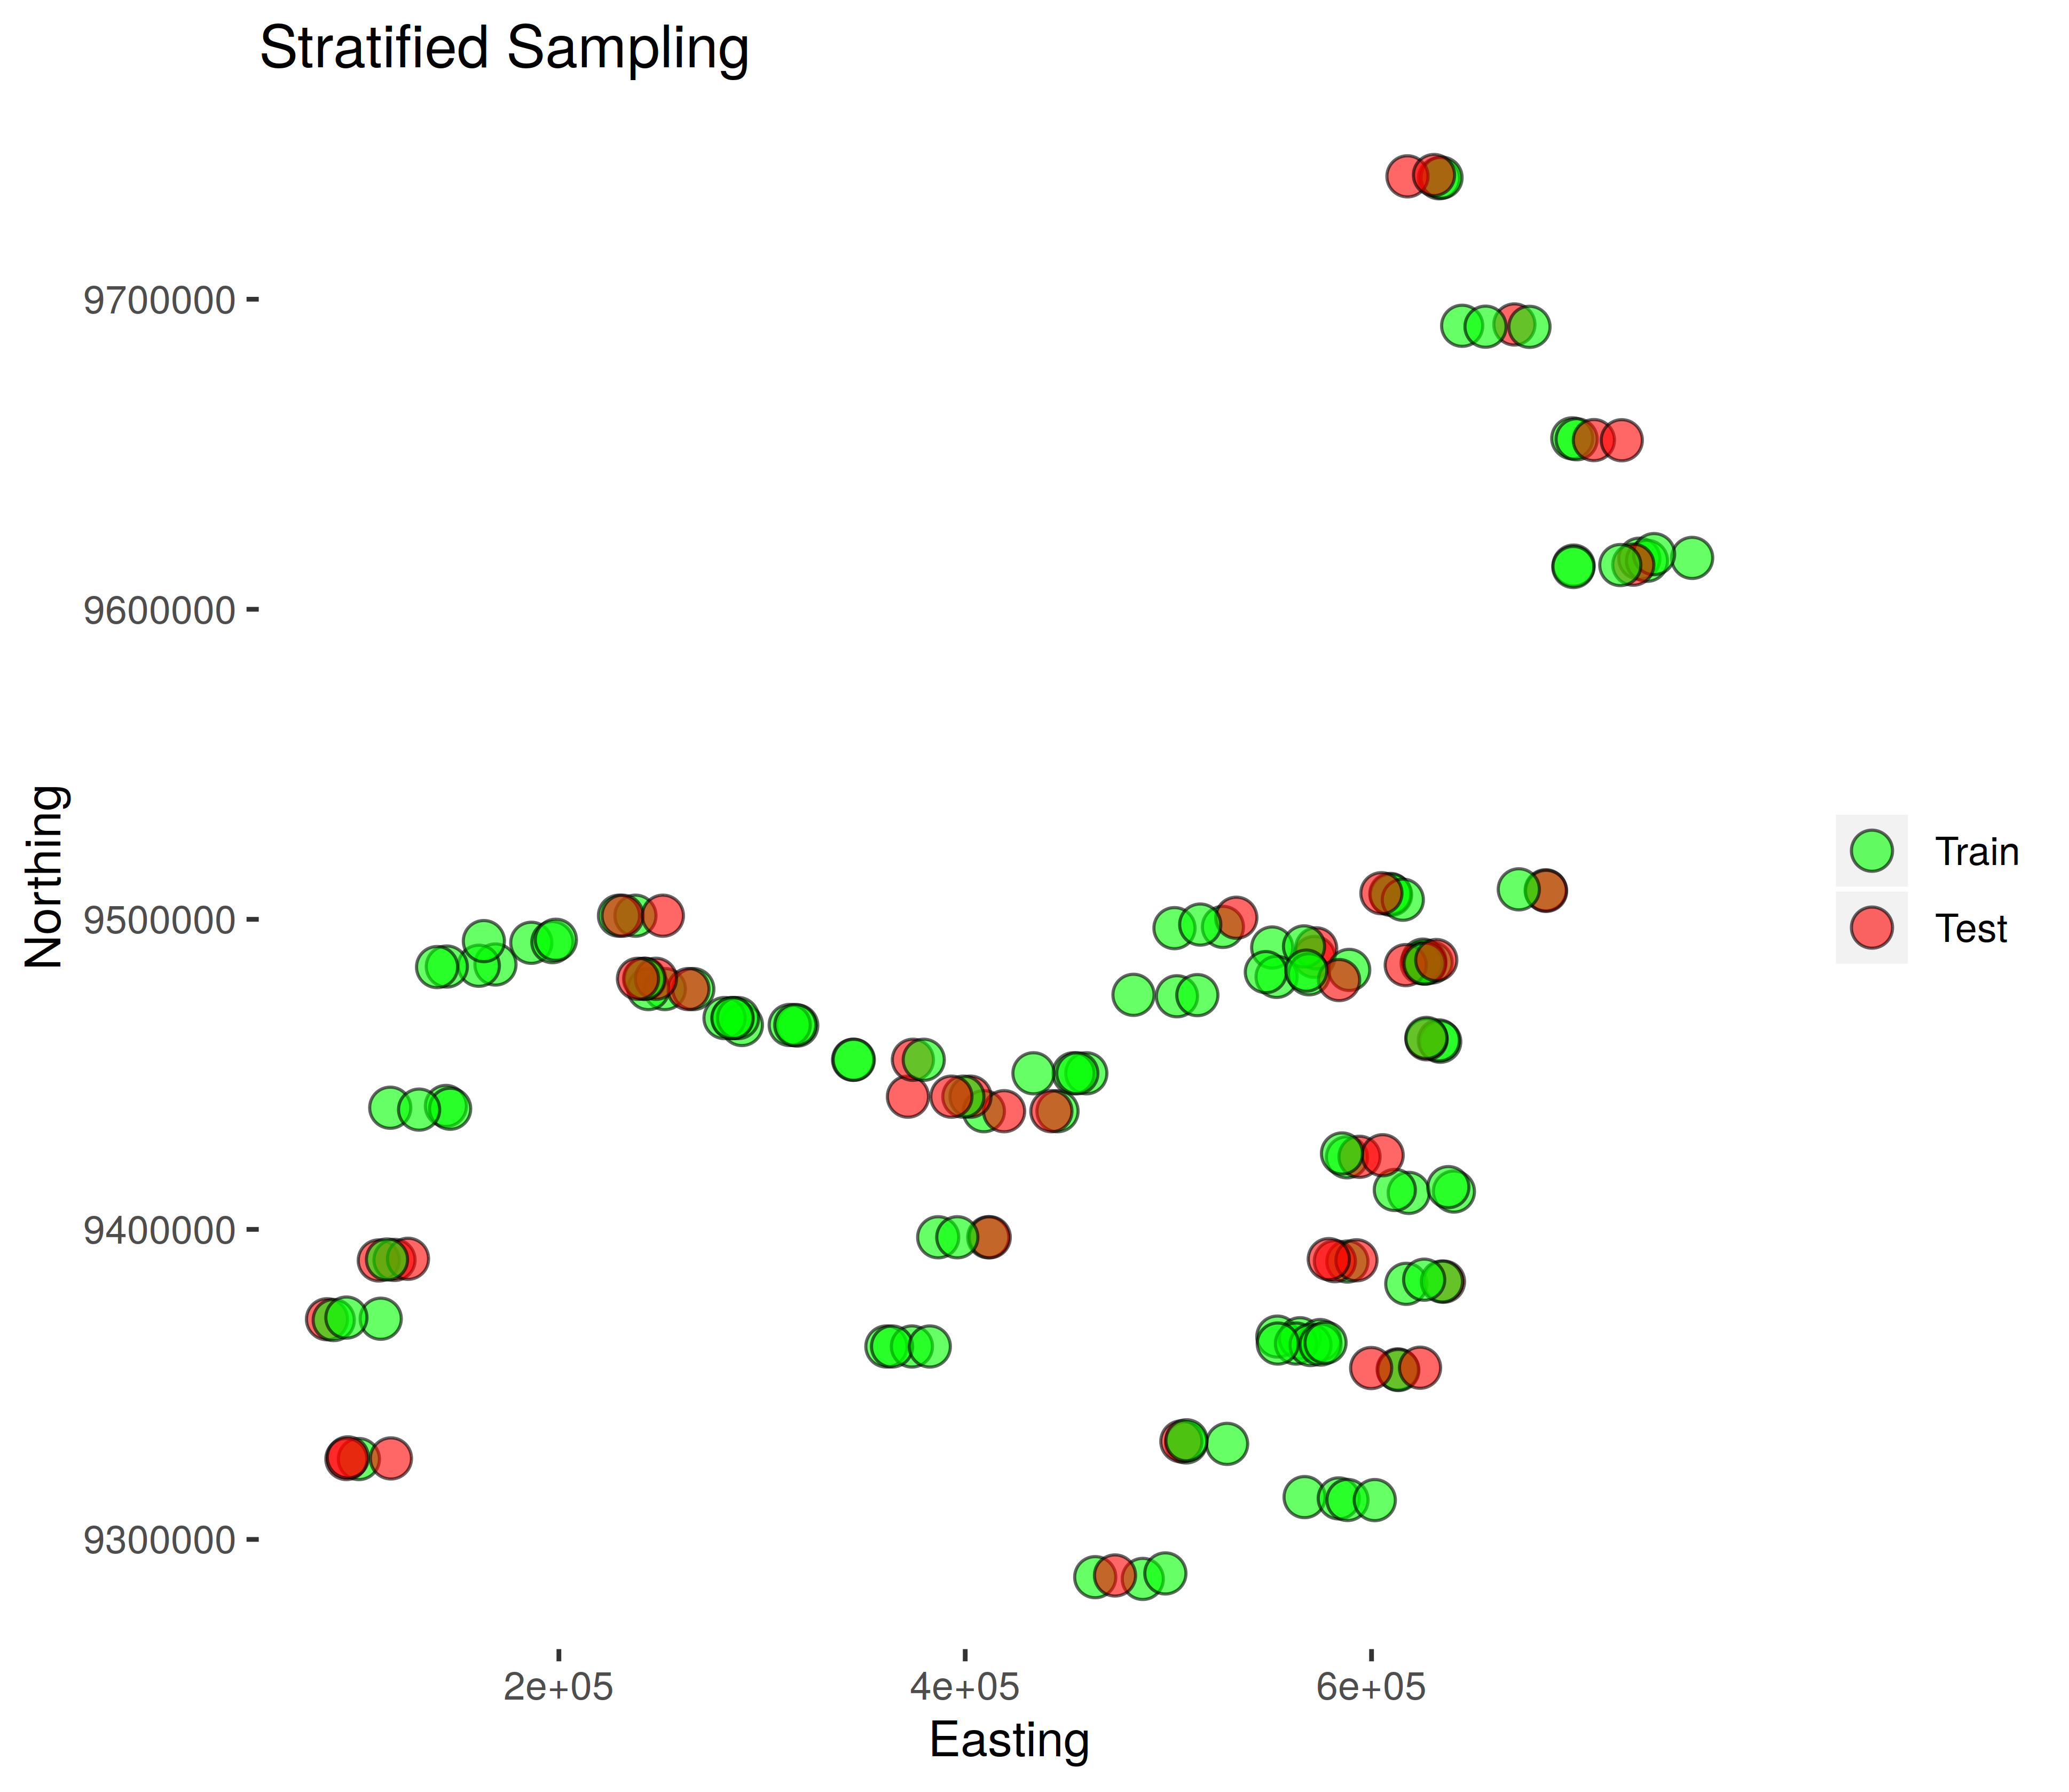
\includegraphics[width = \textwidth]{stratsamp2.png}
\end{subfigure}
\caption{Test set samples are geographically among Train set samples. This represents a maximally similar split which is created by ensuring constant distribution of samples in each part of the river in both the Train and Test set.}
\label{fig:stratsampl}
\end{figure}

%Group sample plot
\begin{figure}[h]
\centering
\begin{subfigure}{0.4\textwidth}
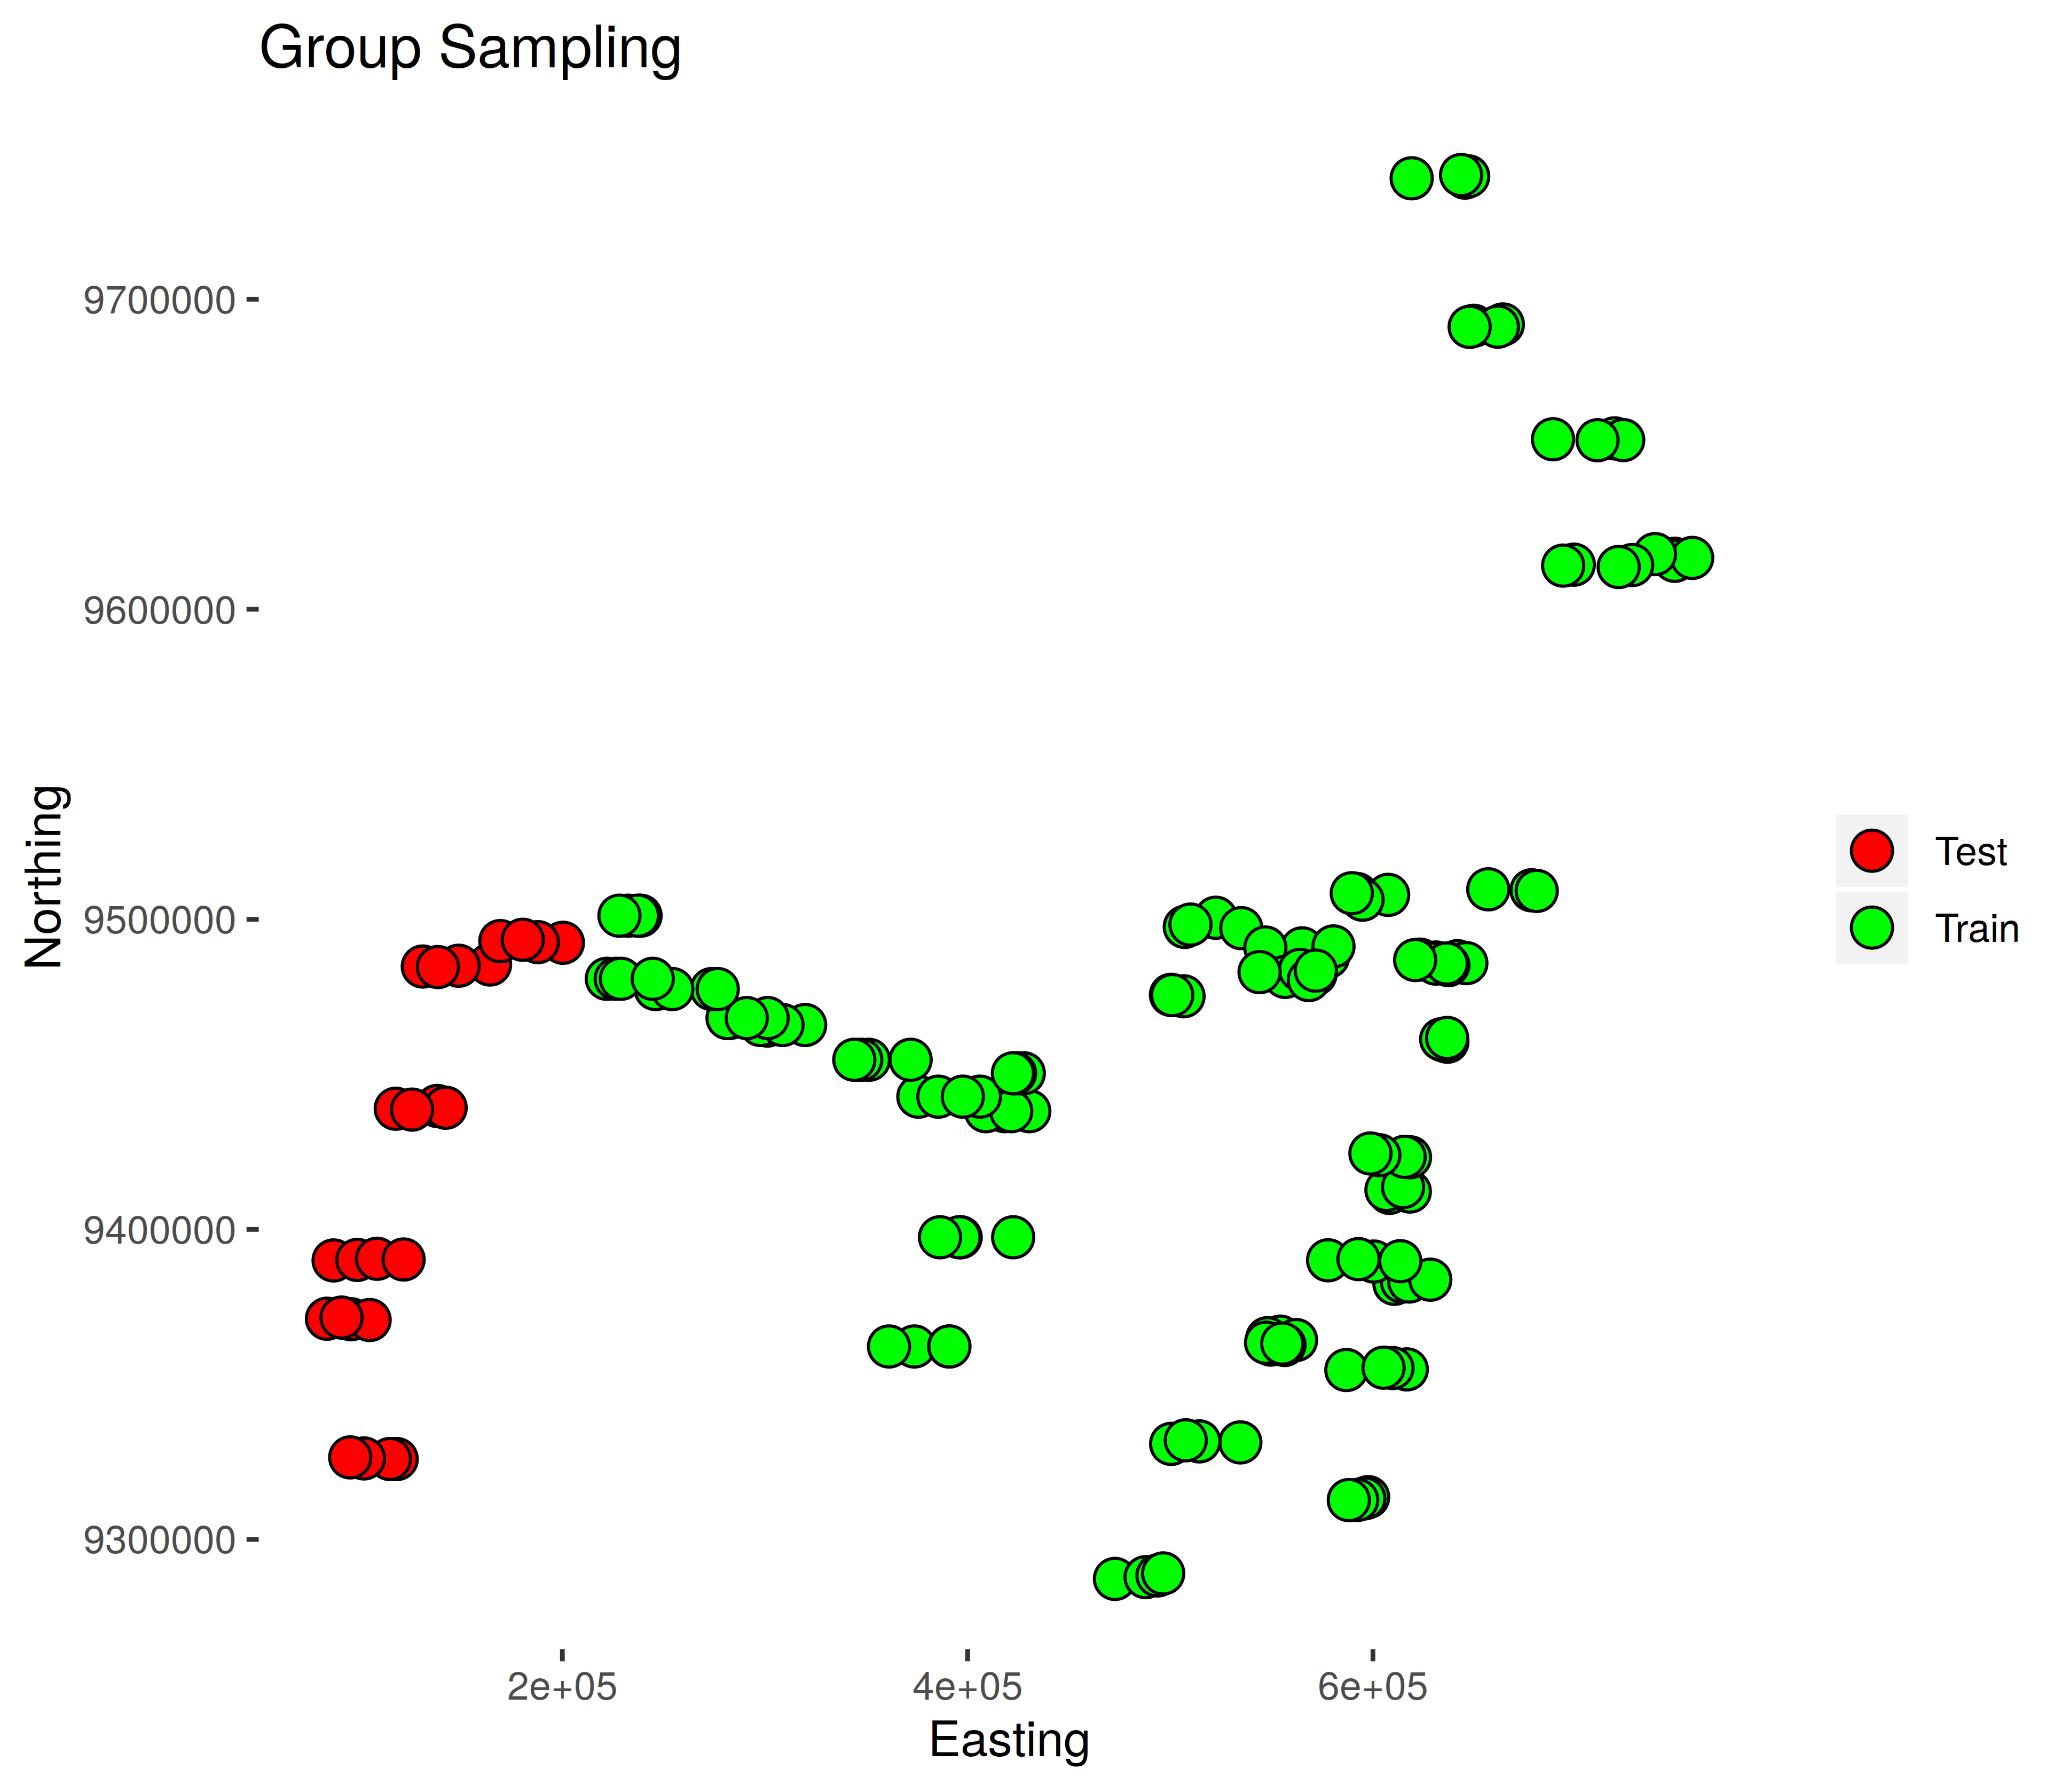
\includegraphics[width = \textwidth]{groupsamp.png}
\end{subfigure}
\begin{subfigure}{0.4\textwidth}
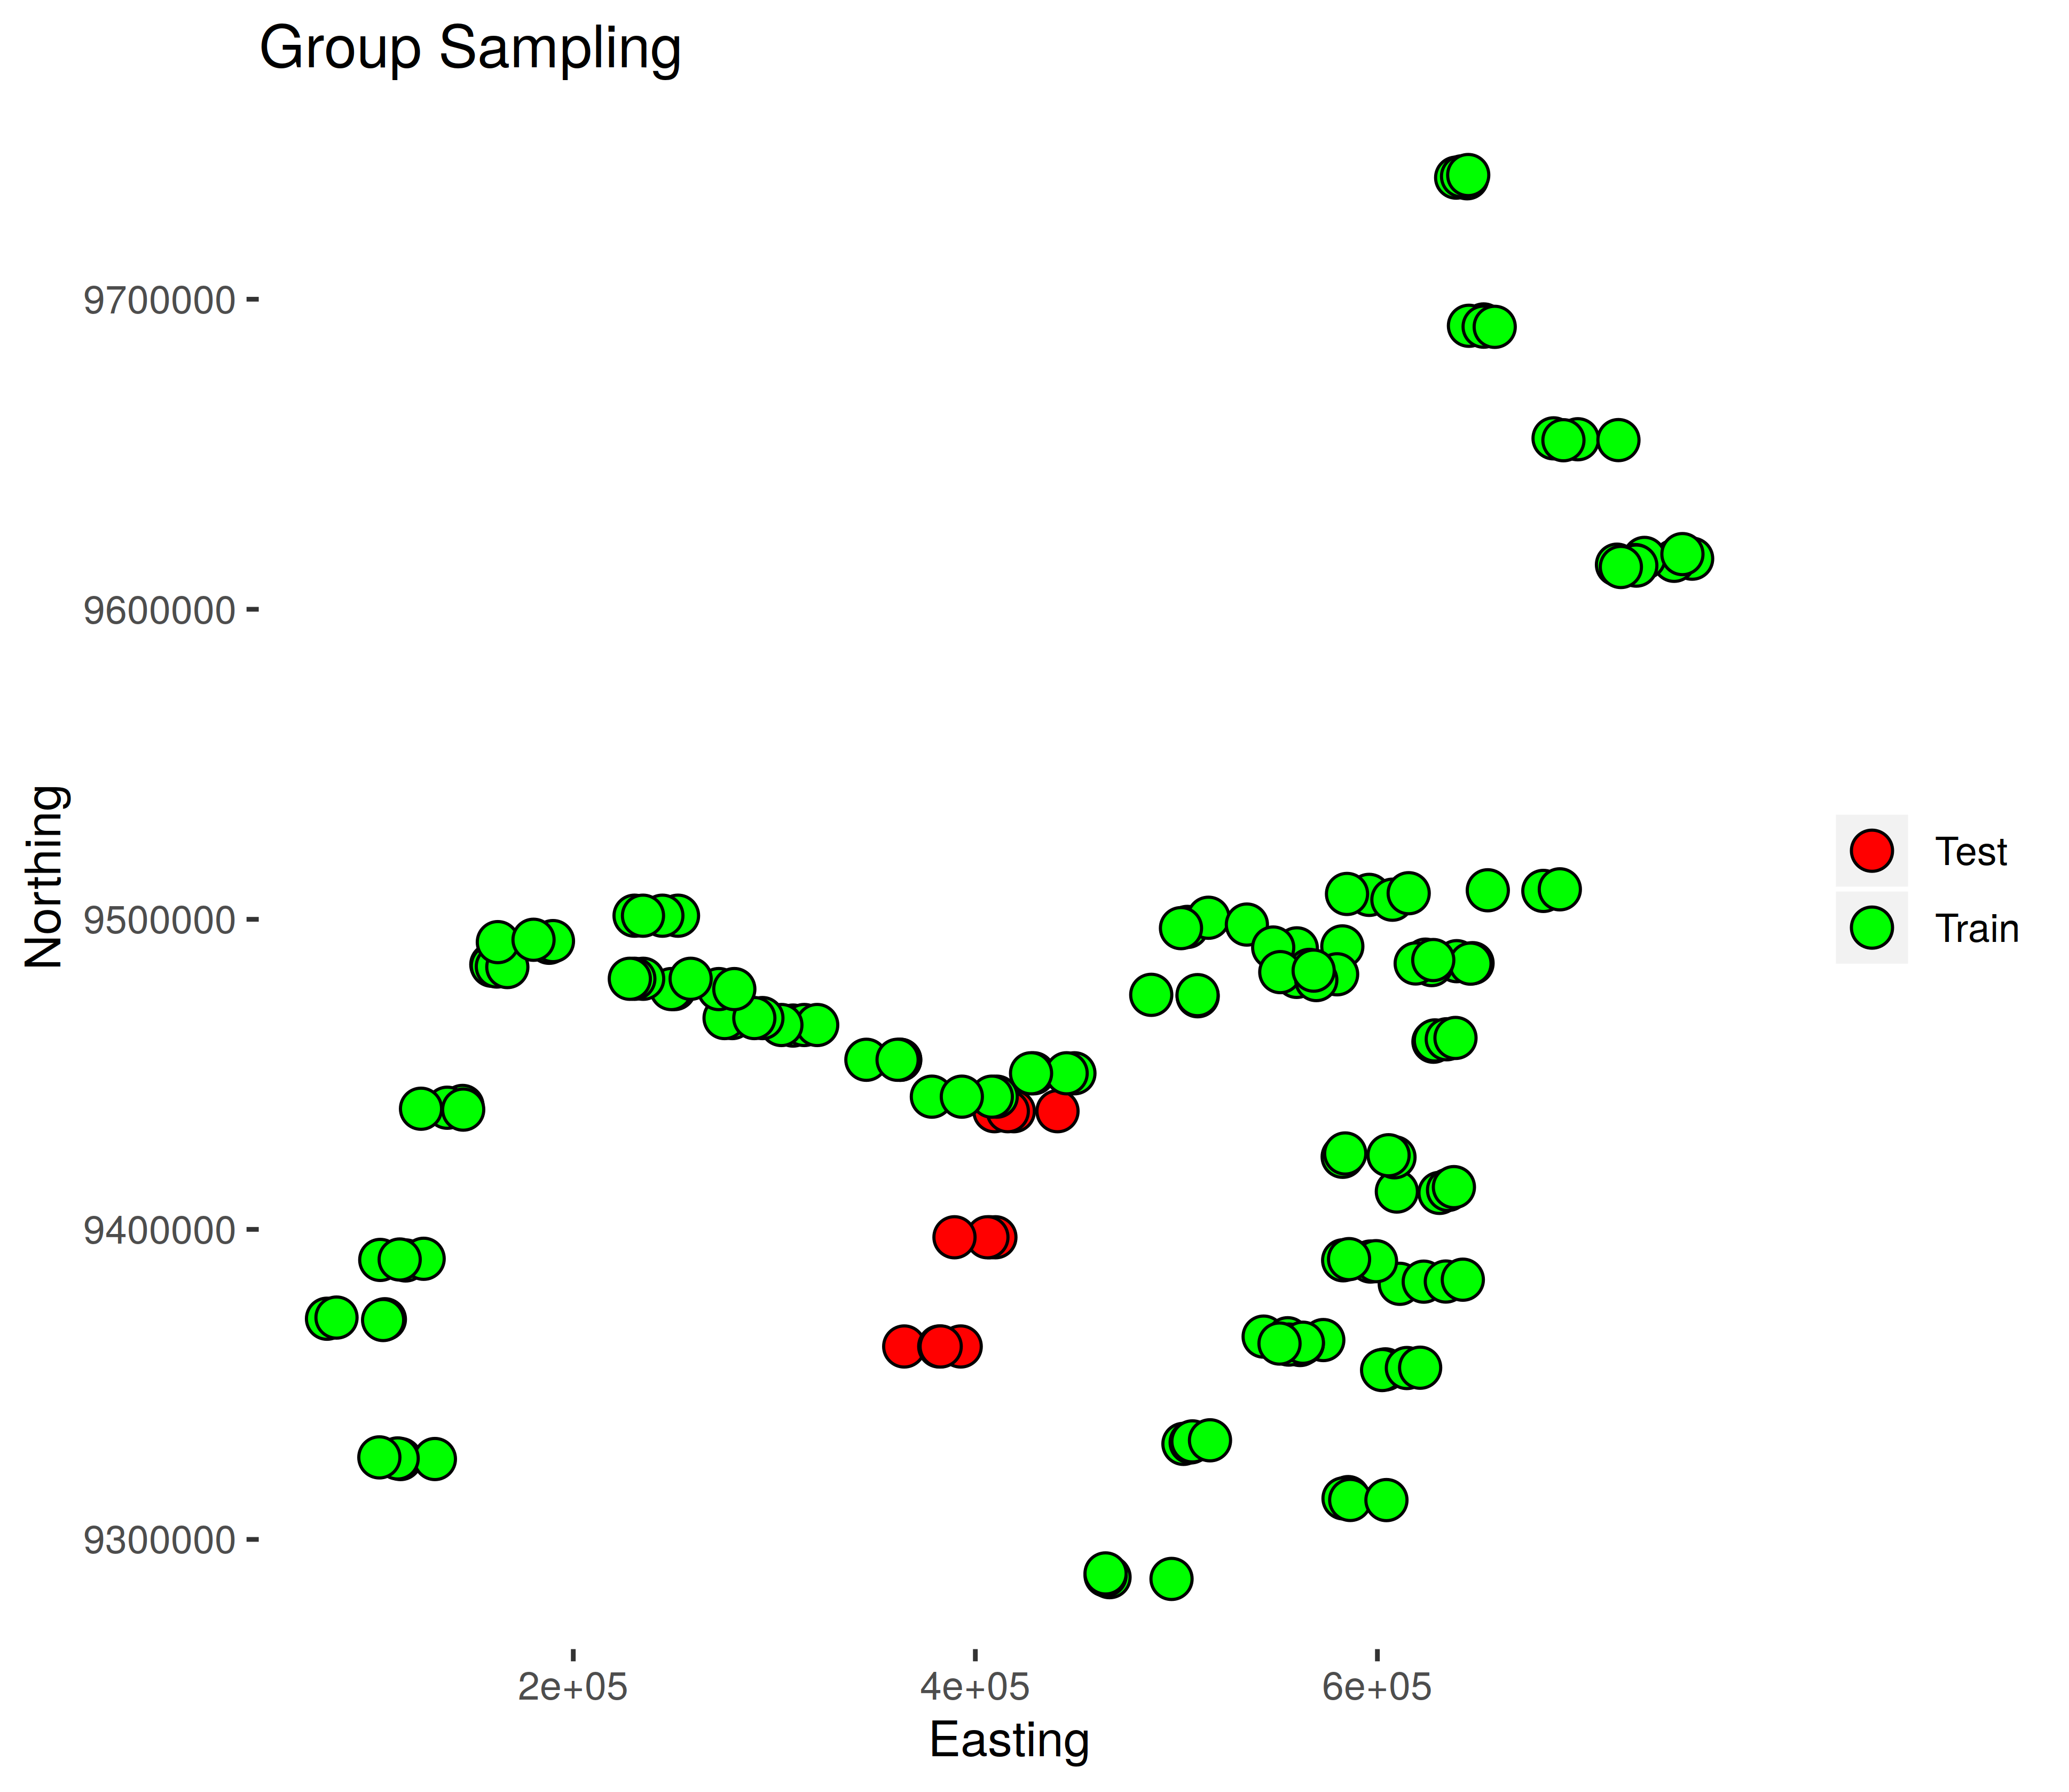
\includegraphics[width = \textwidth]{groupsamp2.png}
\end{subfigure}
\caption{Test set samples are geographically distinct from Train set samples. This represents a maximally dissimilar split which is created by choosing a different part of the river as the Testing set.}
\label{fig:groupsamp}
\end{figure}


To avoid choosing a split method, several ones have been employed that represented different splitting conditions. The classifiers have then been tested on all of them so as to evaluate how well they can perform under various circumstances.

%Validation sets
In addition to splitting the data into training and test sets, the train set was further split into validation sets so as to tune the hyperparameters of the models. The splitting into validation sets followed the same principle/method as the train-test split. So if, for example, the Train and Test sets were split using the maximally similar approach, the validation sets produced from the Train set were chosen so as to be maximally similar to the remaining set.



\subsection{Maximising Similarity}
\textit{Aim}: Evaluate how well the classifiers perform when they are tested on a set which is similar geographically to the train set.
\textit{Method}: Testing and validation sets are made up of samples coming from every part of the river. Care is taken to ensure that no geographical area is over represented. 

To do this Stratified Sampling is used, but instead of keeping the class balance constant in the train validation and test sets we keep the distribution of the samples in the different parts of the rivers constant.

\begin{table}
\caption{Results from maximising similarity using Logistic Regression}
\centering
\label{table:similarity}
\begin{tabular}{l c  c}
\hline 
Features used & Mean Score & Variance of Score \\ 
 
\hline
OTU & 98.2\% & 0.04\%   \\
OTU CSS & 96.2\% & 0.13\%   \\
OTU Min CSS & 96.7\% & 0.11\%   \\
PCoA Bray-Curtis CSS &96.2\% & 0.13\%   \\

\hline 
\end{tabular}
\end{table}


\subsection{Maximising Dissimilarity}

\begin{table}[h]
\caption{Results from maximising dissimilarity using Logistic Regression}
\centering
\label{table:dissimilarity}
\begin{tabular}{l c  c}
\hline 
Features used & Mean Score & Variance of Score \\ 
 
\hline
OTU & 80.7\% & 1.96\%   \\
OTU CSS & 85.7\% & 1.13\%   \\
OTU Min CSS & 84.7\% & 1.4\%   \\
PCoA Bray-Curtis CSS &88.5\% & 1.27\%   \\

\hline 
\end{tabular}
\end{table} 
\subsection{Random Splits}
\dots and some more \dots




\begin{table}
\caption{Even better looking table using booktabs}
\centering
\label{table:good_table}
\begin{tabular}{l c c c c}
\toprule
\multirow{2}{*}{Dental measurement} & \multicolumn{2}{c}{Species I} & \multicolumn{2}{c}{Species II} \\ 
\cmidrule{2-5}
  & mean & SD  & mean & SD  \\ 
\midrule
I1MD & 6.23 & 0.91 & 5.2  & 0.7  \\

I1LL & 7.48 & 0.56 & 8.7  & 0.71 \\

I2MD & 3.99 & 0.63 & 4.22 & 0.54 \\

I2LL & 6.81 & 0.02 & 6.66 & 0.01 \\

CMD & 13.47 & 0.09 & 10.55 & 0.05 \\

CBL & 11.88 & 0.05 & 13.11 & 0.04\\ 
\bottomrule
\end{tabular}
\end{table}



